% !TEX root = main.tex
\renewcommand{\labelenumi}{\alph{enumi})}
\textbf{5. (Dos puntos) ¿Qué es la estandarización de una variable 
aleatoria normal NO estándar, y para qué sirve?}
\\
Cuando una variable aleatoria continua x sigue un adistribuci\'on normal
de media $\mu$ y desviación típica $\sigma$ y se designa por 
$N(\mu, \sigma)$ y esta variable puede tomar su valor de $(\infty, -\infty)$
y su funci\'on de densidad se expresa en t\'erminos de la ecuaci\'on matem\'atica de 
la curva de Gauss:

$F(x) = \frac{1}{\sigma \sqrt{2 \pi}}e^{-\frac{1}{2}(\frac{x -\mu}{\sigma})^{2}}$
\\

\begin{itemize}
    \item El campo de existencia es cualquier valor real, es decir, $(\infty, -\infty)$.

    \item Es simétrica respecto a la media $\mu$.
    
    \item Tiene un máximo en la media $\mu$.
    
    \item Crece hasta la media $\mu$ y decrece a partir de ella.
    
    \item En los puntos $\mu - \sigma$ y $\mu + \sigma$ presenta puntos de inflexión.
    
    \item El eje de abscisas es una asíntota de la curva.
\end{itemize}

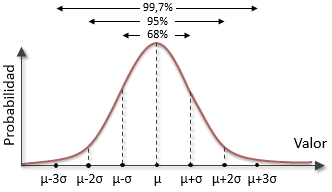
\includegraphics{distNorm.png}

\textbf{Para qu\'e nos sirve la funci\'on de distribuci\'on?} \\

La distribución normal sirve para conocer la probabilidad de encontrar un valor de la variable que sea igual o inferior a un cierto valor , conociendo la media, la desviación estándar, y la varianza de un conjunto de datos en sustituyéndolos en la función que describe el modelo. \\

\textbf{6. ¿Quién dijo la siguiente frase? \\ \\
"Why is raven like a writing desk?" \\
Además, responde la pregunta usando tu imaginación...}
\\ \\
La paregunta aparece en la novela 'Alice's Adventures in Wonderland'
de Lewis Carroll escrita en 1865. En la novela el sombrerero loco
pregunta en una fiesta de te ¿En qu\'e se parece un cuervo a un escritorio?
Y Alice le dice que no tiene idea y el sombrerero dice que el tampoco entonces 
Alice le dice que mejor le de un mejor uso a su tiempo en vez
de tratar de resolver rompecabezas sin soluci\'on.
ALguna gente piensa que es porque Edgar Allan Poe escribi\'o sobre a
ambos. Yo pienso que se asemejan mucho las palabras en frances: bureau y corbeau.
